% Packages
\usepackage{bm,booktabs,tabularx}
\usepackage{animate,soul}
\DeclareUnicodeCharacter{03BC}{$\mu$}
\usepackage{fontawesome}

% Figures
\graphicspath{{figs/}}

% Fonts
\fontsize{13}{15}\sf
\usepackage[scale=0.85]{sourcecodepro}
\DisableLigatures{encoding = T1, family = tt*}
\setbeamerfont{title}{series=\bfseries,parent=structure,size=\fontsize{18}{20}}
\ifcsname Shaded\endcsname
  \definecolor{shadecolor}{RGB}{225,225,225}
  \renewenvironment{Shaded}{\color{black}\fontsize{10}{10}\sf\begin{snugshade}\color{black}}{\end{snugshade}}
\fi

% Colors
\setbeamercolor{description item}{fg=Orange}
\definecolor{MonashBlue}{RGB}{69,88,94}
\definecolor{burntorange}{rgb}{0.8, 0.33, 0.0}

% tikz diagrams
\usepackage{tikz}
\usetikzlibrary{shapes,arrows}
\tikzstyle{decision} = [diamond, draw, fill=blue!20,
    text width=4.5em, text badly centered, node distance=4cm, inner sep=0pt]
\tikzstyle{block} = [rectangle, draw, fill=blue!20,
    text width=5cm, text centered, rounded corners, minimum height=4em]
\tikzstyle{line} = [draw, thick, -latex']
%\tikzstyle{line} = [->,thi
\tikzstyle{cloud} = [draw, ellipse,fill=red!20, node distance=3cm,
    minimum height=2em, text centered]
\tikzstyle{connector} = [->,thick]

% gt dependencies
\usepackage{longtable,caption,setspace}
\captionsetup{font={small,stretch=0.80}}

% My definitions

\def\E{\text{E}}
\def\V{\text{Var}}
\def\up#1{\raisebox{-0.3cm}{#1}}
\def\pred#1#2#3{\hat{#1}_{#2|#3}}
\def\damped{$_\text{d}$}
\def\h+{h_{m}^{+}}
\def\str#1{\rlap{#1}\textcolor{red}{\rule{1cm}{0.1cm}}}

\def\forecast{\begin{alertblock}{}\fontsize{10}{11}\sf
A forecast is an estimate of the probabilities of possible futures.
\end{alertblock}}

\def\simfutures{\begin{textblock}{2.7}(13,7.7)
\begin{block}{}\fontsize{10}{11}\sf
Simulated futures from an ETS model
\end{block}\end{textblock}}

\def\fullwidth#1{\centerline{\includegraphics[height=27.1cm,width=16cm,keepaspectratio=true]{#1}}}
\def\fullheight#1{\centerline{\includegraphics[height=7.65cm,width=25cm,keepaspectratio=true]{#1}}}
\def\full#1{\centerline{\includegraphics[height=7.7cm,width=15cm,keepaspectratio=true]{#1}}}

% Title page graphic
  \titlegraphic{
    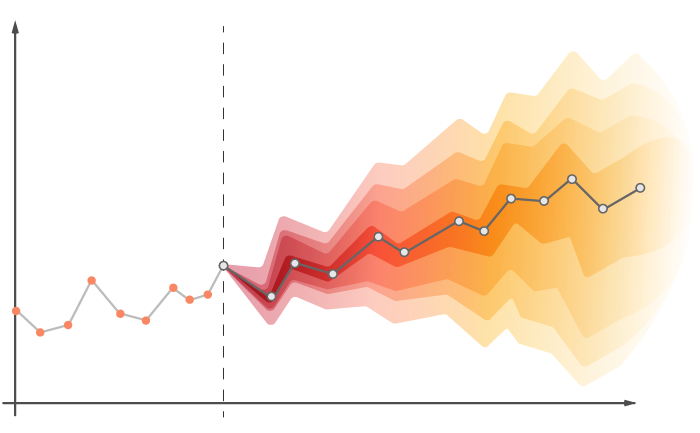
\includegraphics[height=1.5in]{./Images/probabilistic-forecasting-graph.png} \vspace{1in}
  }
  
  % Vanderbilt color scheme
  \usepackage{xcolor}
  \definecolor{gold}{RGB}{207,174,112}  % gold
  \definecolor{black}{RGB}{10,10,10} % black
  \definecolor{white}{RGB}{255,255,255} % white
  \setbeamercolor{title}{fg = gold}
  \setbeamercolor{title}{bg = black}
  \setbeamercolor{normal text}{fg = black}
  \setbeamercolor{frametitle}{fg = gold}
  \setbeamercolor{frametitle}{bg = black}
  \setbeamercolor{structure}{fg = gold}
  \setbeamercolor{structure}{bg = black}
  \setbeamercolor{item}{fg = black}
  
  % Other stuff
  \usepackage{amssymb}
  \usepackage{ragged2e}
  \usepackage{multicol}
  \usepackage{mwe}
  \usepackage{textpos}
  
  % Default setup
  \usepackage[sfdefault]{cabin}
  \usepackage{hyperref}
  %\hypersetup{
  %  colorlinks = true,
  %  allcolors = blue
  %}
  \usepackage{float, placeins}
  \usepackage{booktabs}
  
  % Additional packages
  \usepackage[edges]{forest}
  
  % tikz equation packages
  \usepackage{tikz}
  \usetikzlibrary{backgrounds}
  \usetikzlibrary{tikzmark}
  \usetikzlibrary{calc}
  \usetikzlibrary{arrows,shapes,positioning,shadows,trees,mindmap}
  \usetikzlibrary{arrows.meta}
  \colorlet{linecol}{black!75}
  \usepackage{xkcdcolors} % xkcd colors

  % Basic equation packages
  \usepackage{amsmath}
  \usepackage{amsthm}
  \usepackage{amssymb}
  \usepackage{mathtools}
  \usepackage{nccmath}
  \usepackage{wrapfig}
  \usepackage{comment}
  \usepackage{blindtext}
  \usepackage{graphicx}
  \usepackage{xspace}
  \usepackage{array}
  \usepackage{ragged2e}
  \newcolumntype{P}[1]{>{\RaggedRight\hspace{0pt}}p{#1}}
  \newcolumntype{X}[1]{>{\RaggedRight\hspace*{0pt}}p{#1}}
  \DeclarePairedDelimiter{\norm}{\lVert}{\rVert}


  % Color packages
  \usepackage{xcolor}
  \usepackage{tcolorbox}
  \newcommand{\highlight}[2]{\colorbox{#1!30}{$\displaystyle #2$}}
  \newcommand{\highlightdark}[2]{\colorbox{#1!50}{$\displaystyle #2$}}
  \renewcommand{\highlight}[2]{\colorbox{#1!30}{#2}}
  \renewcommand{\highlightdark}[2]{\colorbox{#1!50}{#2}}
  
  % Define colors
  \definecolor{red}{HTML}{F03D2D}
  \definecolor{skyblue}{HTML}{90DDF0}
  \definecolor{green}{HTML}{C8D96F}
  \definecolor{orange}{HTML}{EF8A17}
  \definecolor{yellow}{HTML}{F5C900}
  \definecolor{purple}{HTML}{BA42C0}
  \definecolor{teal}{HTML}{17BEBB}
  \definecolor{greyblue}{HTML}{9BAFD9}

